% !TeX spellcheck = en_GB
\documentclass[10pt,letterpaper,oneside]{article}
\usepackage{fontspec}
\usepackage{arev}
\usepackage[utf8]{inputenc}
\usepackage[T1]{fontenc}
\usepackage{amsmath}
\usepackage{amsfonts}
\usepackage{amssymb}
\usepackage{graphicx}
\usepackage{csquotes}
\usepackage{booktabs}
\usepackage{multicol}
\usepackage{enumerate}
\usepackage{microtype}
\usepackage[labelfont=bf,font={small}]{caption}
\usepackage{hyperref}
\usepackage{booktabs}
\usepackage{subcaption}
\usepackage{fancyhdr}
\usepackage[svgnames]{xcolor}
\usepackage{mdframed}
\usepackage{multicol}
\usepackage[para]{footmisc}
\usepackage{siunitx}
\usepackage{cleveref}
\usepackage{listings}
\usepackage{cprotect}


\lstset{ % General setup for the package
	language=Python,
	basicstyle=\small\ttfamily,
	tabsize=4,
	columns=fixed,
	showstringspaces=false,
	showtabs=false,
	keepspaces,
	commentstyle=\color{SeaGreen},
	keywordstyle=\bf\ttfamily\color{DarkBlue}
}

\newfontfamily\symbolfont{Symbola}
\usepackage[left=1in,right=1in,top=1in,bottom=1in,marginparwidth=0.3in]{geometry}

\usepackage[sorting=none]{biblatex}
\addbibresource{../bibliography.bib}

\author{Andreas Stöckel\\[0.5cm]Based on lecture notes by\\Chris Eliasmith and Terrence~C.~Stewart}
\newcommand{\baseCodeURL}{https://github.com/astoeckel/syde556-w20/blob/master/lectures}

\fancyhf{}
\fancyhead[L]{SYDE 556/750 Lecture Notes}
\fancyhead[R]{Andreas Stöckel}
\fancyfoot[C]{\thepage}
\pagestyle{fancy}

\setlength{\parindent}{0em}
\setlength{\parskip}{0.5em}
\renewcommand{\baselinestretch}{1.25}
\renewcommand{\vec}[1]{{\mathbf{#1}}}
\newcommand{\mat}[1]{{\mathbf{#1}}}
\newcommand{\T}{\ensuremath{\mathrm{T}}}
\renewcommand{\epsilon}{\varepsilon}
\renewcommand{\phi}{\varphi}

\makeatletter
\newcommand{\superimpose}[2]{%
	{\ooalign{{#1}\hidewidth\cr{#2}\hidewidth\cr}}}
\makeatother
\newcommand{\SolidCircle}[2]{\superimpose{\color{#1}\symbolfont ⬤}{\textbf{\color{white}#2}}\hspace{1em}}
\newcommand{\OPlus}{\SolidCircle{DarkGreen}{\kern0.75pt+}}
\newcommand{\OMeh}{\SolidCircle{DarkOrange}{~}}
\newcommand{\OMinus}{\SolidCircle{DarkRed}{\kern2.25pt--}}

\newcommand{\YouTube}[2][Video]{\href{https://youtu.be/#2}{{\symbolfont 📺}~{#1}}%
%\footnote{\url{https://youtu.be/#2}}%
}

\newcommand{\CodeLink}[2][Code]{\href{\baseCodeURL/#2}{{\symbolfont ⌨}~\emph{#1}}}

\newcommand{\MakeTitle}[1]{
\maketitle
\begin{center}
	
\includegraphics[width=0.5\textwidth]{../assets/uwlogo.pdf}\\[1cm]
	{#1}\
\end{center}

\vfill

\thispagestyle{empty}
\setcounter{page}{0}
\newpage

\pagenumbering{roman}
\setcounter{tocdepth}{2}
\tableofcontents
\newpage

\setcounter{page}{0}
\pagenumbering{arabic}}

\reversemarginpar


\newcommand{\ColorBox}[3]{%
	\marginpar{%
		\huge\raisebox{-3ex}{\symbolfont{#1}}%
	}%
	\begin{mdframed}[hidealllines=true,backgroundcolor=#2,innertopmargin=0.25cm,innerbottommargin=0.25cm]%
		{#3}
	\end{mdframed}}

\newcommand{\Note}[1]{\ColorBox{📌}{WhiteSmoke}{\textbf{Note:} #1}}
\newcommand{\Example}[1]{\ColorBox{💡}{WhiteSmoke}{\textbf{Example:} #1}}
\newcommand{\Aside}[1]{\ColorBox{🌟}{WhiteSmoke}{\emph{Aside:} #1}}
\newcommand{\Python}[1]{\ColorBox{🐍}{WhiteSmoke}{#1}}
\newcommand{\Notation}[1]{\ColorBox{\huge$\Sigma$}{WhiteSmoke}{\textbf{Notaton:} #1}}

\newcommand{\ConstructionSite}{\hrulefill {\symbolfont 🚧} UNDER CONSTRUCTION {\symbolfont 🚧} \hrulefill}

\newenvironment{ImportantEqn}[1]{\mdframed\raggedleft\emph{({#1})}\align}{\endalign\endmdframed}

\date{January 14 \& 16 \& 21, 2020}
\title{SYDE 556/750 \\ Simulating Neurobiological Systems \\ Lecture 3: Representation}


\begin{document}

\MakeTitle{\textbf{Accompanying Readings: Chapter 2 of Neural Engineering}}

\section{Introduction}

\Note{In the last lecture, we had a look at a the Leaky Integrate-and-Fire neuron model as an approximation of the behaviour of biological neurons. In this lecture, we discuss a theory of neural representation. Together, these two ideas will give us a theory of what \enquote{the neural code} may be.}

In order to survive in natural environments, animals must build representations of their surroundings. This includes the physical properties of objects in their vicinity, such as \emph{velocity}, \emph{location}, \emph{colour}, etc., but also non-physical properties such as whether an object is \emph{edible}, or \emph{dangerous}. Of course such representations are not only limited to external objects, but may carry information about the own body (e.g., \enquote{proprioception}, configuration of limbs; location in space), up to abstract thought and emotions.

For now, and mostly because it is the easiest to reason about, we shall restrict ourselves to relatively low-level representations of sensory information. In this case, the fact that a neuron is representing an external quantity is directly evident from correlation between the quantity and the neuron's activity.  We saw examples of such representations in the first lecture. For example, in the classical Hubel and Wiesel experiment (\YouTube{KE952yueVLA}, \cite{hubel1959receptive}), neural activity is correlated with the location and orientation of a bar of light (an \enquote{edge}) within the visual field. Similarly, in the case of place cells (\YouTube{lfNVv0A8QvI}), neural activity is correlated with the location of the animal in space.

A central claim of the Neural Engineering Framework (NEF) is that values $\vec x$ -- e.g., the physical quantities mentioned above -- are represented in the neural activity $\vec a$ of \emph{groups} of neurons. Furthermore, we claim that there is a non-linear encoding process that translates a value into a neural activity pattern, and a linear decoding process that estimates the represented value from neural activity patterns.

\begin{mdframed}
\textbf{NEF Principle 1 -- Representation}\\
\emph{Groups} (\enquote{populations}, or \enquote{ensembles}) of neurons \emph{represent} values via nonlinear encoding and linear decoding.
\end{mdframed}

We will first discuss the encoding and decoding of values in a more abstract sense, and then propose a particular mechanism by which values are encoded in the NEF. Since \emph{encoding} only takes us half of the way, we then discuss \emph{decoding}, in particular in the presence of noise in the neural activities.

\Notation{Scalars, functions are italic letters ($d$, $n$, $N$, $f$,\textellipsis), vectors are bold lowercase letters ($\vec a, \vec e$, $\vec x$), matrices are bold uppercase letters ($\mat A$), sets are double-struck uppercase letters ($\mathbb{R}$, $\mathbb{N}$). $\mathbb{A} \rightarrow \mathbb{B}$ denotes a function mapping from the domain $\mathbb{A}$ onto a codomain $\mathbb{B}$.
\allowdisplaybreaks
\begin{align*}
	d &\in \mathbb{N} &&~ \text{Dimensionality of the value represented by a neuron population} \\
	n &\in \mathbb{N} &&~ \text{Number of neurons in a neuron population} \\
	N &\in \mathbb{N} &&~ \text{Number of samples}\\
	\langle \vec x, \vec y \rangle &: \mathbb{R}^k \times \mathbb{R}^k \rightarrow \mathbb{R} &&~ \text{Dot product between two $k$-dimensional vectors $\vec x$ and $\vec y$} \\¸
	G[J]  &: \mathbb{R} \rightarrow \mathbb{R}^+  &&~ \text{Neural response for an input current $J$ (\emph{response curve})} \\
	a_i (\vec x) &: \mathbb{R}^d \rightarrow \mathbb{R}^+ &&~ \text{Neural response of neuron $i$ in a neural population (\emph{tuning curve})}\\
	\vec a(\vec x) &: \mathbb{R}^d \rightarrow (\mathbb{R}^+)^n &&~ \text{Neural response of all neurons in a neural population}\\
	{\vec e}_i &\in \mathbb{R}^d &&~ \text{Encoding vector, or \enquote{preferred direction}, of neuron $i$ in a population}\\
	\alpha_i &\in \mathbb{R} &&~ \text{The $i$-th neuron's gain factor}\\
	J^\mathrm{bias}_i &\in \mathbb{R} &&~ \text{The $i$-th neuron's bias current}\\
	\vec x_j &\in \mathbb{R}^d &&~ \text{$j$-th (out of $N$) input sample} \\
	{\hat{\vec x}}_j &\in \mathbb{R}^{d} &&~ \text{Decoded $j$-th input sample} \\
	\mat X &\in \mathbb{R}^{d \times N} &&~ \text{Matrix of input samples}\\
	\mat A &\in \mathbb{R}^{n \times N} &&~ \text{Matrix of sampled population activities}\\
	\vec d_i &\in \mathbb{R}^{n} &&~ \text{Decoding vector for the $i$-th neuron in the population} \hspace{0.25cm}\\
	\mat D &\in \mathbb{R}^{d \times n} &&~ \text{Decoding matrix}
\end{align*}\vspace{-0.75cm}}

\section{Codes: Representing Information}

Human societies have relied on exchanging coded information for millennia. Apart from written and spoken language themselves, examples of such codes include flag semaphores, or Morse code \cite{2009itur}.

These codes have in common that there is some kind of \emph{encoding} process that turns an original message $\vec x$ into a coded message $\vec a$, and a \emph{decoding} process that reconstructs $\vec x$ from $\vec a$. If $\vec x$ can be perfectly reconstructed, this is called \emph{lossless coding}, otherwise \emph{lossy coding}.

\subsection{Lossless Codes}

In the case of a lossless code, there exists an encoding function $f$, as well as its inverse $f^{-1}$. It holds
\begin{align*}
	\vec a &= f(\vec x) \,, && \text{Encoding} \\
	\vec x &= f^{-1}(\vec a) = g(f(\vec x)) \,. && \text{Decoding} 
\end{align*}

\paragraph{Morse Code} Morse code is an example of such a lossless coding scheme. A function $f$ takes a character sequence and turns it into valid Morse code, consisting of dots~($\cdot$) and dashes~($-$):
\begin{align*}
	\begin{aligned}
	f&: \mathcal{S}(\{\mathtt{A}, \ldots, \mathtt{Z}, \text{\textvisiblespace}\}) \rightarrow \mathbb{M} \,, \\
	f^{-1} &: \mathbb{M} \rightarrow \mathcal{S}(\{\mathtt{A}, \ldots, \mathtt{Z}, \text{\textvisiblespace}\}) \,,
	\end{aligned} &&\quad \text{where } \mathbb{M} \subset \mathcal{S}(\{\cdot, -\}) \text{ is the set of valid Morse messages} \,.
\end{align*}
Here, $\mathcal{S}$ denotes the set of all sequences consisting of the given elements (i.e., the union over all Cartesian powers).

\paragraph{Binary numbers}
As a more concrete example, let's consider an $n$-bit binary coding of natural numbers. Here, our coded message $\vec a = (a_0, a_1, a_2, a_3, \ldots, a_{n - 1})$ where $a_i \in \{0, 1\}$, while our original value $x$ is a natural number between zero and $2^n - 1$.

We can write down the encoding function $f$
\begin{align*}
	a_i &= \big(f(x)\big)_i = \begin{cases}
		1 & \text{if } x - 2^i \left\lfloor \frac{x}{2^i} \right\rfloor > 2^{i - 1} \,,\\
		0 & \text{otherwise} \,.
	\end{cases}
\end{align*}
This function is nonlinear -- we cannot write it as a matrix-vector product. The decoding function $f^{-1}$ is given as
\begin{align*}
	x &= f^{-1}(\vec a) = \sum_{i=0}^{n -1} 2^i a_i \,.
\end{align*}
This function is \emph{linear} in $\vec a$ because we can write it as a matrix-vector product
\begin{align*}
x = f^{-1}(\vec a) = {\mat F} \vec a = \begin{pmatrix} 1 & 2 & \ldots & 2^{n - 1}\end{pmatrix} \begin{pmatrix} a_0 \\ a_1 \\ \vdots \\ a_{n - 1} \end{pmatrix} \,.
\end{align*}
Since a single value $x$ is represented in multiple \enquote{units} (here: digits of a binary number), we call this kind of coding scheme a \emph{distributed} representation.

\Note{A precise definition of \emph{linearity} is provided in the notes for Lecture 2.

We could imagine using such a binary coding scheme in the context of a neural network. In a population of $n$ neurons, each neuron $i$ would represent one binary digit. However, there are several problems with this approach.
\begin{itemize}
	\item Individual units represent vastly different magnitudes. Since biological neural networks are noisy and we are using a linear decoding scheme, noise in the unit representing the digit $i = 8$ is amplified by a factor of $256$ compared to noise in the unit representing the digit $i = 0$.
	\item We assume that our units can only have two possible values, zero and one, whereas neural units can have graded responses (cf.~the response curve $G[J]$).
	\item The encoding function is quite complicated. There is no neurophysiological evidence that brains use a binary coding scheme.
\end{itemize}}

\subsection{Lossy Codes}

In contrast to lossless codes, lossy codes have no perfect inverse $f^{-1}$. Instead, we have a decoding function $g$ that \emph{approximates} the original value. Mathematically, we have
\begin{align*}
	\vec a &= f(\vec x) \,, && \text{Lossy Encoding} \\
	\vec x &\approx g(\vec a) = g(f(\vec x)) \,. && \text{Lossy Decoding} 
\end{align*}

\paragraph{Examples of lossy codes} In mathematics and engineering, examples of such lossy codes include Principal Component Analysis (PCA; nonlinearly reduces a dataset onto its first $n$ principal basis vectors), and coding schemes for audio and images, such as MP3 and JPEG (these coding schemes are based on the Discrete Cosine Transformation).

\Aside{Surprisingly, the Discrete Cosine Transformation (DCT) turns out to be a close to optimal \emph{linear} transformation for the compression of natural signals. When computing the PCA of a large corpus of natural images or audio (the PCA optimally ensures that the most variance in the data is explained by the first dimensions), the resulting linear transformation is very similar to the DCT. However, the DCT of a signal $\vec x$ can be computed more efficiently (in $\mathcal{O}(d \log(d))$) compared to a general linear transformation (in $\mathcal{O}(d^2)$).}

\section{Neural Representation}

As discussed in the introduction, there are some neuron populations in the brain that directly represent information about stimuli in the environment. In order to better understand these representations, we first have a look at so called \emph{tuning curves}, mappings between external stimuli and the neural activity.

After looking at some real-world data, we combine our observations into a general encoding equation that captures as many properties of tuning curves as possible.

\Note{The coding scheme we are using for neural representation is both \emph{distributed} and (in practice) \emph{lossy}. In contrast to binary coding, our distributed coding scheme is more resilient to noise in the neural activities $\vec a$. Lossyness mostly stems from neurons having a limited dynamic range (saturation effects) and -- although this is not an inherent problem of the coding scheme itself -- noise in the neural system.}

\subsection{Neural Tuning Curves}

\begin{figure}[p]
	\begin{subfigure}[b]{0.5\textwidth}%
		\centering%
		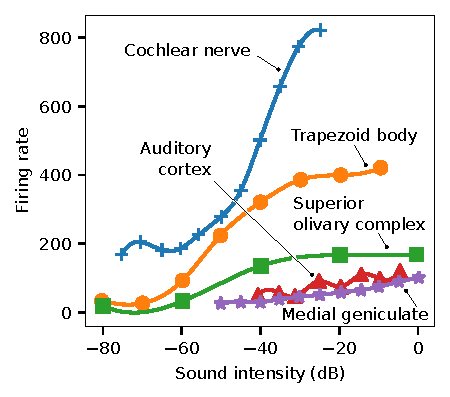
\includegraphics{media/audition_tuning_curves_annotated.pdf}%
		\caption{Neural tuning curves for auditory processing}%
		\label{fig:audition_tuning_curves_annotated}%
	\end{subfigure}
	\begin{subfigure}[b]{0.5\textwidth}%
		\centering%
		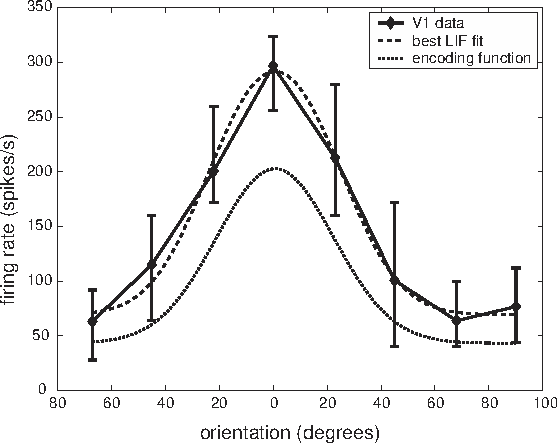
\includegraphics[width=\textwidth]{media/eliasmith_et_al_2003_orientation_tuning.pdf}%
		\caption{Visual orientation tuning in V1.}
		\label{fig:eliasmith_et_al_2003_orientation_tuning}
	\end{subfigure}
	\caption{\textbf{(a)} Neural firing rates in different brain regions involved in auditory processing as a function of sound intensity in cats. Figure adapted from \cite{mann1997nervous} (Chapter 8), data from \cite{katsuki1969neural}. \CodeLink[Code used to plot the data]{lecture_03/media/code/audition.ipynb}. \textbf{(b)} Example of visual orientation tuning of a cell in primary visual cortex of a macaque monkey. Figure copied from \cite{eliasmith2003neural}, fig.~3.1.}
	\label{fig:tuning_curves_1}
\end{figure}

\begin{figure}[p]
	\hspace{0.5cm}
	\begin{subfigure}[b]{0.25\textwidth}%
		\centering%
		\hspace{-1cm}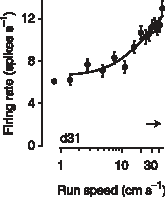
\includegraphics[scale=1.4]{media/saleem_et_al_tuning_curves_a.pdf}%
		\caption{}%
		\label{fig:saleem_et_al_tuning_curves_a}%
	\end{subfigure}%
	\begin{subfigure}[b]{0.25\textwidth}%
		\centering%
		\hspace{-1cm}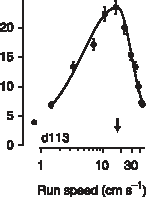
\includegraphics[scale=1.4]{media/saleem_et_al_tuning_curves_b.pdf}%
		\caption{}%
		\label{fig:saleem_et_al_tuning_curves_b}%
	\end{subfigure}%
	\begin{subfigure}[b]{0.25\textwidth}%
		\centering%
		\hspace{-1cm}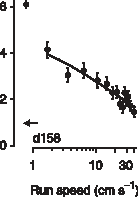
\includegraphics[scale=1.4]{media/saleem_et_al_tuning_curves_c.pdf}%
		\caption{}%
		\label{fig:saleem_et_al_tuning_curves_c}%
	\end{subfigure}%
	\begin{subfigure}[b]{0.25\textwidth}%
		\centering%
		\hspace{-1cm}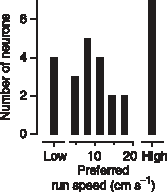
\includegraphics[scale=1.4]{media/saleem_et_al_tuning_curves_d.pdf}%
		\caption{}%
		\label{fig:saleem_et_al_tuning_curves_d}%
	\end{subfigure}%
	\caption{Tuning curves of individual neurons in visual cortex (layer V1) for mice running in the dark. \textbf{(a-c)} Neural firing rates over the running speed of the mouse. \textbf{(d)} Histogram over tuning curve types. Figures copied from \cite{saleem2013integration}.}
	\label{fig:tuning_curves_2}
\end{figure}

In the last lecture, we have discussed neural \emph{response curves}. Response curves are a mapping between the current $J$ injected into a neuron and the corresponding neural activities. \emph{Tuning curves} are a similar concept. However, instead of plotting the current $J$ over the neural response, we plot some varying (external) stimulus over the neural response. \Cref{fig:tuning_curves_1,fig:tuning_curves_2} depict neural tuning curves as found in the neuroscience literature.

\Note{Tuning curves and \emph{internal} stimuli. Neuroscientists usually define tuning curves as the relationship between an \emph{external} stimulus and the neural response. In the NEF we extend this concept towards internal stimuli, i.e.,~neurons representing purely internal states, such as short-term memory. The lack of such tuning curves in the literature may be purely attributed to it being very hard to experimentally capture these relationships.}

Overall, we can qualitatively distinguish between three types of tuning curves (cf.~\cref{fig:saleem_et_al_tuning_curves_d})
\begin{enumerate}[i.]
	\item Responses that \emph{increase} with the intensity of the stimulus (stimulus and neural response are positively correlated; cf.~\cref{fig:audition_tuning_curves_annotated,fig:saleem_et_al_tuning_curves_a}).
	\item Responses that \emph{decrease} with the intensity of the stimulus (stimulus and neural response are negatively correlated; cf.~\cref{fig:saleem_et_al_tuning_curves_c}).
	\item Responses that have a \emph{preferred stimulus}; their response is maximal if the stimulus has a certain value and decreases if the value deviates from that value (cf.~\cref{fig:saleem_et_al_tuning_curves_b,fig:eliasmith_et_al_2003_orientation_tuning}).
\end{enumerate}

Tuning curves of type \emph{i.}~can be easily explained by rescaling and offsetting the neural input current $J$ to match the data. In other words, we have a simple \emph{current translation function} $J_i(x)$ that converts the stimulus $x$ into a current $J$ that is being injected into the $i$-th neuron of our population:
\begin{align}
	J_i(x) &= \alpha_i x + J^\mathrm{bias}_i \,,
	\label{eqn:current_translation_scalar}
\end{align}
where $\alpha_i$ is the so called \emph{gain factor} and $J^\mathrm{bias}_i$ is the \emph{bias}. These parameters are different for each neuron in the population and model the diverse neural responses of individual neurons within the same brain area. Tuning curves of type \emph{ii.}~can be generated by choosing a negative gain $\alpha_i$.

\Example{You can try to find parameters that qualitatively match the tuning curves in \cref{fig:tuning_curves_1,fig:tuning_curves_2} by playing around with the gain and offset parameters in \CodeLink[this Jupyter Notebook]{lecture_03/media/code/tuning_curve_experiments.ipynb}.}

This leaves us with tuning curves of type \emph{iii.}, i.e.~tuning curves having a preferred value. We generate these tuning curves by extending the current translation function \cref{eqn:current_translation_scalar} to accepting vectorial quantities as input.

\subsection{The Encoding Equation}

In order to generate tuning curves that qualitatively match all types of tuning curves we have seen above, we let our value $\vec x$ be a $d$-dimensional vector. The dimensionality of the represented value $d$ is specific to each neuron population. We can then choose the dot product as a measure of similarity (see note below):
\begin{align*}
	J_i(\vec x) &= \alpha_i \langle \vec x, \vec e_i \rangle + J^\mathrm{bias}_i \,,
\end{align*}
where $\alpha_i$, $J^\mathrm{bias}_i$ are the gain and bias terms for the $i$-th neuron in the population, $\vec e_i \in \mathbb{R}^d$ is the neuron's encoding -- or \enquote{preferred direction vector}, and $\langle \cdot, \cdot \rangle$ denotes the dot product between two vectors. Note that $\vec e_i$ is always normalised to unit length, that is $\|\vec e_i\| = 1$.

\Note{The \emph{dot product} (also: inner product, scalar product) $\langle \vec x, \vec y \rangle$ of two vectors $\vec x, \vec y \in \mathbb{R}^d$ is defined as
	\begin{align*}
	\langle \vec x, \vec y \rangle &= \sum_{i = 0}^d x_i y_i \,.
	\end{align*}
	We implicitly treat all vectors as column vectors; a vector $\vec x \in \mathbb{R}^d$ is implicitly a $d \times 1$ matrix (i.e., a matrix of $d$ rows and a single column). Hence, by the definition of matrix multiplication, the dot product is also given as
	\begin{align*}
	\langle \vec x, \vec y \rangle &= \vec x^\T \vec y  \quad \text{(matrix dimensions: $(1 \times d) \times (d \times 1) \rightarrow (1 \times 1)$)}\,.
	\end{align*}
	In particular, note that the dot product can be interpreted as a vector similarity measure. Namely, according to the Euclidean dot product formula
	\begin{align*}
	\langle \vec x, \vec y \rangle &= \cos(\angle(\vec x, \vec y)) \| \vec x\| \| \vec y\| \,,
	\end{align*}
	where $\| \cdot \|$ denotes the standard $L_2$-norm, and $\angle(\cdot, \cdot)$ is the angle inscribed between two vectors. Hence, the dot product is maximal if the angle between the two vectors is zero (they are pointing in the same direction, the cosine is $+1$) and zero if the two vectors are orthogonal. It is minimal (the cosine is $-1$) if the two vectors are pointing in exactly opposite directions.}

Combining the current $J_i(\vec x)$ with the neuron response curve $G[J]$ (where, again, $G$ is specific to each neuron population) yields the \enquote{encoding equation}, which describes the nonlinear representational encoding process performed by each neuron within a population
\begin{ImportantEqn}{Encoding Equation}
	a_i(\vec x) &= G\big[J_i(\vec x)\big] = G\big[\alpha_i \langle \vec x, \vec e_i \rangle + J^\mathrm{bias}_i\big] \,.
	\label{eqn:encoding}
\end{ImportantEqn}

\paragraph{Example: 1D Encoder}
In the case of a one-dimensional encoder, the encoding \enquote{vector} can either be $+1$ or $-1$. This corresponds to o neurons that are either more active in the presence of a stimulus (positive encoder), or neurons that are more active in the absence of a stimulus (negative encoder).

\begin{figure}
	\begin{subfigure}{0.5\textwidth}
		\centering
		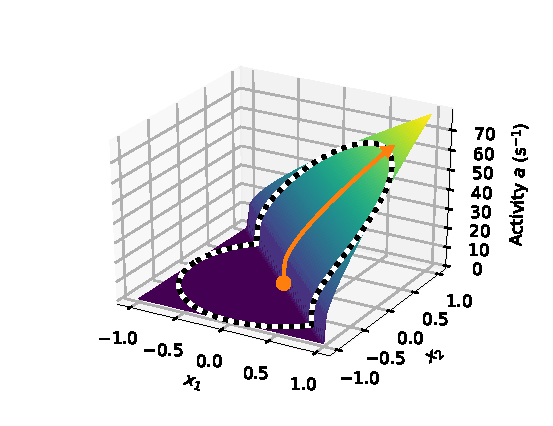
\includegraphics[trim=1cm 0 0 1cm,clip]{media/2d_encoder_tuning_curve.pdf}
		\caption{2D neuron tuning curve}
		\label{fig:2d_encoder_tuning_curve}
	\end{subfigure}
	\begin{subfigure}{0.5\textwidth}
		\centering
		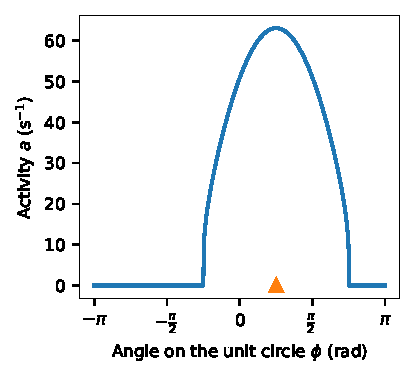
\includegraphics{media/2d_encoder_tuning_curve_unit.pdf}
		\caption{1D projection along the unit circle}
		\label{fig:2d_encoder_tuning_curve_unit}
	\end{subfigure}
	\caption{2D neuron tuning curve for the encoding vector $\vec e = (1/\sqrt{2}, 1/\sqrt{2})$. \textbf{(a)} 3D surface plot of the 2D neuron tuning curve. Axes correspond to the magnitude of the first two components of the represented value $\vec x = (x_1, x_2)$. Orange arrow corresponds to the encoding vector. Dotted line corresponds to the unit circle. \textbf{(b)} Neural activity along the unit circle is qualitatively similar to the bell-shaped tuning curves observed in biology. \CodeLink{lecture_03/media/code/2d_encoder.ipynb}}
\end{figure}

\paragraph{Example: 2D Encoder}
\Cref{fig:2d_encoder_tuning_curve_unit} shows a tuning curve in a 2D representational space. Note that moving along the unit-circle in 2D-space generates the \enquote{preferred direction} tuning curve type observed in nature.

\section{Decoding Represented Values}

As we have seen in the binary coding example above, some codes possess a \enquote{complex}, non-linear encoding scheme, but can be decoded using a simple linear decoder. Neuroscientists have similarly found that they can use a simple linear decoding scheme to extract represented values from neural populations -- we will later discuss some more examples.

In general, having a linear decoder means that we can estimate the value $\hat{\vec x}$ represented by a neural population by multiplying its current activity $\vec a$ with a decoding matrix $\mat D$:
\begin{align*}
	(\vec a)_i &=
		G\big[\alpha_i \langle \vec x, \vec e_i \rangle + J^\mathrm{bias}_i\big] \,, && \text{Encoding} \\
	\hat{\vec x} &= \mat D \vec a \,. && \text{Decoding}
\end{align*}

In the special case of a population representing a scalar value (i.e.,~the represented dimensionality $d = 1$) we have
\begin{align*}
(\vec a)_i &=
G\big[\alpha_i \langle x, e_i \rangle + J^\mathrm{bias}_i\big] \,, && \text{Encoding} \\
\hat{x} &= \langle \vec d, \vec a \rangle = \sum_{i = 1}^n d_i a_i \,. && \text{Decoding}
\end{align*}

Now that we now how to decode the represented value $\vec x$ \emph{in principle}, we of course have to somehow compute these decoders.


\subsection{Computing Identity Decoders}

In order to compute the decoders, we first have to think about what the decoders should optimally do. The roles of the decoders is to estimate the represented value. In the optimal case we would like the decoded value $\hat{\vec x}$ to be equal to or as close as possible to the encoded value $\vec x$. That is, in general, we would like to minimize the error $E$ (also called a \emph{loss function})
\begin{align}
	\arg\min_{\mat D} E = \int_{\mathbb{X}} \|\vec x - \hat{\vec x}\| \,\mathrm{d}\vec x = \int_{\mathbb{X}} \|\vec x - \mat D \vec a(\vec x)\| \,\mathrm{d}\vec x \,,
	\label{eqn:optimisation_problem}
\end{align}
where $\mathbb{X}$ is a compact subspace of the possible represented values in $\mathbb{R}^d$ we are interested in.

\newpage

\Note{The dynamic range of a neural representation is limited due to neural saturation and noise -- it is not possible to represent all real numbers in a single neuron population. This is why we are using this \enquote{weird} integral over a subspace $\mathbb{X}$ -- we must restrict ourselves to a range of numbers we want to be able to decode well.
	
The quantifier \emph{compact} is just a mathematical technicality that ensures that $\mathbb{X}$ is actually a \enquote{closed range} we can integrate over, and not just individual vectors picked from $\mathbb{R}^d$.}

\paragraph{Mathematical derivation} In order to make the math a little more digestible, assume that we want to find the decoders for scalar represented values ($d = 1$) and that the represented values we are interested in are over the interval $\mathbb{X} = [-1, 1]$. The above equation becomes
\begin{align}
	\arg\min_{\vec d} E
		&= \arg\min_{\vec d} \int_{-1}^1 \sqrt{ \left(x - \langle \vec d, \vec a(x) \rangle\right)^2 } \,\mathrm{d}x
		 = \arg\min_{\vec d} \frac{1}2 \int_{-1}^1 \left(x - \sum_{i = 1}^n d_i a_i(x) \right)^2 \,\mathrm{d}x \,.
	\label{eqn:decoder_loss}
\end{align}
This equality holds because eliminating the square root and adding a factor $\frac{1}2$ does not change the location of the minimum. Since this is a quadratic equation we know that there is exactly one extremum. In this particular case, we also know that this extremum must be a minimum (since the quadratic term has a positive sign). Hence, we can find the $\vec d$ that minimizes the error by differentiating with respect to individual $d_i$ and setting the derivative to zero:
\begin{align*}
	\frac{\partial E}{\partial d_i}
		&= \frac{1}2 \int_{-1}^1 2 \left(x - \sum_{j = 1}^n d_j a_j(x) \right) \left(-a_i(x) \right) \,\mathrm{d}x
		 = \int_{-1}^1 \sum_{j = 1}^n a_j(x) d_j a_i(x) \,\mathrm{d}x - \int_{-1}^1 a_i(x) x \,\mathrm{d}x
		\overset{!}= 0 \,.
\end{align*}
Rearranging yields the following equality at $\frac{\partial E}{\partial d_i} = 0$:
\begin{align*}
	\int_{-1}^1 a_i(x) x \,\mathrm{d}x
		&= \int_{-1}^1 \sum_{j = 1}^n a_j(x) d_j a_i(x) \,\mathrm{d}x
		 = \sum_{j = 1}^n d_j \left( \int_{-1}^1 a_j(x) a_i(x) \,\mathrm{d}x \right) \,.
\end{align*}
Upon closer inspection we see that this is a system of $n$ linear equations over $\vec d = (d_1, \ldots, d_n)$. Hence, we can write this in matrix notation as $\mat\Upsilon = \mat\Gamma \vec d$, where
\begin{align*}
	\left( \mat\Upsilon \right)_i
		&= \int_{-1}^1 a_i(x) x \,\mathrm{d}x \,, &
	\left( \mat\Gamma \right)_{ij}
		 = \int_{-1}^1 a_j(x) a_i(x) \,\mathrm{d}x \,.
\end{align*}
Further evaluation of the integrals is -- generally speaking -- not possible in closed form. What we can do however is to approximate the integrals by (randomly) sampling. We pick $N$ sample points $x_1, \ldots, x_N$. Then, the above equation becomes (approximately)
\begin{align*}
	\frac{1}N \sum_{k = 1}^N a_i(x_k) x_k
		&= \frac{1}N \sum_{j = 1}^n d_j \sum_{k = 1}^N a_j(x_k) a_i(x_k) \,.
\end{align*}
The factor $1/N$ accounting for the discretisation of the integral cancels out. In matrix notation, letting $(\mat A)_{ik} = a_i(x_k)$ and $\vec \xi = (x_1, \ldots, x_k)$ we get
\begin{align*}
	\vec d &=\mat \Gamma^{-1} \mat \Upsilon \approx  (\mat A \mat A^T)^{-1} \mat A \vec \xi^\T \,, &&
	\text{where } \mat \Upsilon \approx \mat A \vec \xi \text{ and } \mat \Gamma \approx \mat A \mat A^\T \,.
\end{align*}

In general, solving \cref{eqn:optimisation_problem} directly (i.e.,~without assuming $d = 1$ and $\mathbb{X} = [-1, 1]$), we get
\begin{ImportantEqn}{Computing decoders without taking noise into account}
	\mat D^\T &\approx  (\mat A \mat A^T)^{-1} \mat A \mat X^\T \,.
	\label{eqn:decoders}
\end{ImportantEqn}
Here, $A = \big(\vec a(\vec x_1), \ldots \vec{(\vec x_N)}\big)$ is a matrix containing the population activities as column vectors for each sample ${\vec x}_k$. $\mat X = ({\vec x}_1, \ldots, {\vec x}_k)$ is a matrix containing each input sample as a column vector.

\begin{figure}
	\centering
	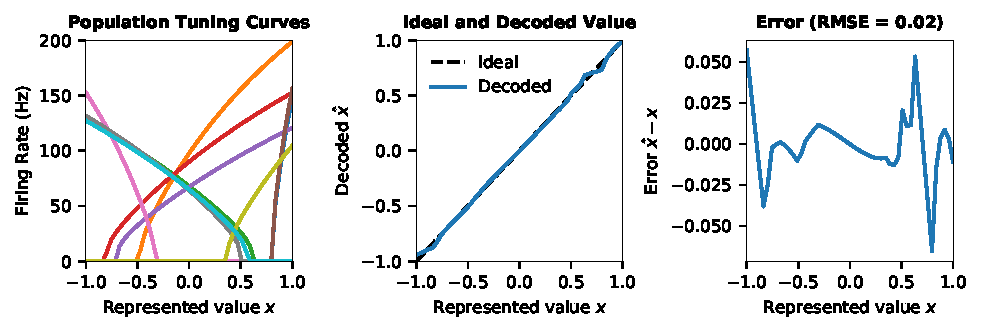
\includegraphics{media/decoding_example_no_noise.pdf}
	\caption{Example of decoding the represented values from a population of neurons. \emph{Left:} Tuning curves for a population of ten neurons. Tuning curves were chosen such that the $x$-intercepts of the tuning curves are sampled from a uniform distribution over the interval $[-1, 1]$. The maximum firing rate over that interval is uniformly sampled from $[100, 200]$. Neuron encoders were randomly selected to be either $+1$ or $-1$. \emph{Middle:} Represented value and the decoded value on the same plot. \emph{Right:} Decoding error $\hat x - x$. \CodeLink{lecture_03/media/code/computing_decoders.ipynb}}
	\label{fig:decoding_example_no_noise}
\end{figure}

To summarize, in order to solve for decoders we first randomly sample a set of $N$ values $\mat X = ({\vec x}_1, \ldots, {\vec x}_k)$ we would like to represent. Using the encoding equation in \cref{eqn:encoding} we then compute what the population activities would be for each of these samples, giving us $A = \big(\vec a(\vec x_1), \ldots \vec{(\vec x_N)}\big)$. We then plug these matrices into \cref{eqn:decoders}, giving us the decoding matrix $\mat D$. \Cref{fig:decoding_example_no_noise} shows an example depicting the overall encoding and decoding process.

\Note{\emph{Least squares.}
The problem we just solved is a \emph{linear least squares optimisation problem}, and the solution given in \cref{eqn:decoders} has been independently discovered in the early 19th century by the mathematicians Adrien-Marie Legendre and Carl Friedrich Gauss.}

\Note{\emph{Moore-Penrose Pseudo Inverse.}
The term \enquote{$(\mat A \mat A^T)^{-1} \mat A$} is also called Moore-Penrose Pseudo Inverse of a matrix $\mat A$. It is sometimes written as $\mat A^+$. The name \enquote{Pseudo Inverse} stems from the fact that it performs an inverse-like operation for non-square matrices.}

\cprotect\Python{In Python, you can solve the above linear least-squares problem using the following code:
\begin{lstlisting}[language=python]
import numpy as np
A = np.array(...) # n x N array
X = np.array(...) # d x N array
D = np.linalg.lstsq(A.T, X.T, rcond=None)[0].T
\end{lstlisting}
Have a look at the \href{https://docs.scipy.org/doc/numpy/reference/generated/numpy.linalg.lstsq.html}{documentation of \texttt{lstsq}} for a precise description of its behaviour.}

\subsection{Sources of Noise in Neural Systems}

We now know how to compute linear decoders $\mat D$ that estimate the value represented by an ensemble of neurons. However, we implicitly made the assumption that each neuron perfectly implements its response curve $G[J]$. We know that this is not true in biological systems.

\paragraph{Noise due to spike rate estimation errors}
The response curve $G[J]$ is only a first-order approximation of a neuron's behaviour. We know that in real biological systems neurons communicate using spikes -- and it is impossible to perfectly estimate it's firing rate over a short time window (cf.~the time and frequency uncertainty principle \cite{gabor1946theory}). This measurement error can be interpreted as \emph{noise}.

\paragraph{Biological sources of error}
Nervous systems contain various sources of error, including, but not limited to the following (cf.~\cite{gerstner2002spiking}, Chapter 5.1)
\begin{itemize}
	\item \textbf{Axonal jitter.}
	The action potential transmission speed varies between spikes. This is because action potentials are transported \emph{actively}, i.e.,~they do not travel along the axon due to passive electrical properties of the axon, but are constantly renewed at the so called \enquote{Nodes of Ranvier}.
	\item \textbf{Neurotransmitter vesicle release failure.}
	Only 10-30\% of pre-synaptic spikes generate a post-synaptic event -- one reason being that the release of neurotransmitter vesicles is stochastic.
	\item \textbf{Amount of neurotransmitter per vesicle.}
	The amount of neurotransmitters in a vesicle varies between vesicles. The intensity of the post-synaptic response depends on the specific vesicle that releases neurotransmitter into the synaptic cleft.
	\item \textbf{Ion channel noise.}
	The excitatory and inhibitory post-synaptic currents are generated by ion-channels in the neuron's cell membrane opening and closing in response to receiving neuro transmitters. These ion-channels are binary: they can either be fully open or fully closed. The graded nature of post-synaptic currents stems from the fact that many ion-channels open and close in a stochastic fashion.
	\item \textbf{Thermal noise.}
	In general, on the level of molecular biology, many processes rely on stochastic events triggered by thermal noise -- this can be seen as an explanation of the noisiness of -- among others -- the above processes.
	\item \textbf{Network effects.}
	Even simple, non-noisy recurrent networks of excitatory and inhibitory spiking neurons can produce highly irregular spike patterns.
\end{itemize}

Given these considerations, we should add a zeroth principle to the NEF:\footnote{In the text this principle is called an \enquote{addendum} and listed as the fourth principle. I think that this principle is so fundamental that it should be number zero in the list.}
\begin{mdframed}
	\textbf{NEF Principle 0 -- Noise}\\
	Biological neural systems are subject to significant amounts of noise from various sources. Any analysis of such systems must take the effects of noise into account.
\end{mdframed}

\begin{figure}
	\centering
	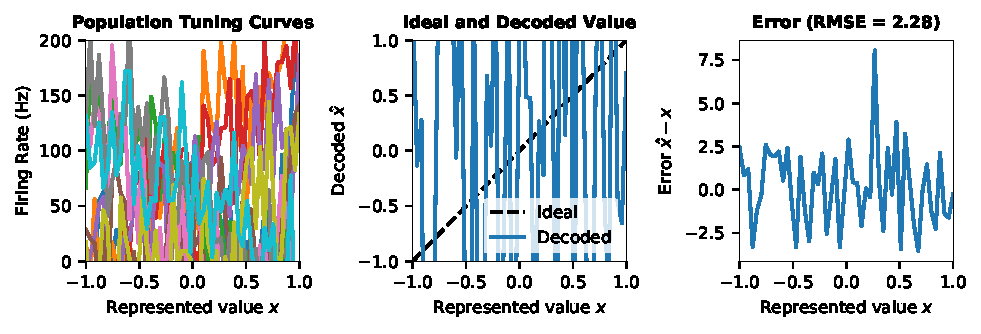
\includegraphics{media/decoding_example_noise.pdf}
	\caption{Decoding the represented value from a population of neurons with added noise (Gaussian, $\mu = 0$, $\sigma = 0.1 \max(A)$). See \cref{fig:decoding_example_no_noise} for the complete description. \CodeLink{lecture_03/media/code/computing_decoders.ipynb}}
	\label{fig:decoding_example_noise}
\end{figure}


\paragraph{Modelling Noise}
To test whether our modelling framework still holds when we take noise into account, we should somehow be able to include noise to our models. There are two potential ways how we can accomplish this. Either we add more detail to our neuron models and simulate the noise sources, or we -- for now -- simply add noise from a distribution to our neural activities $\vec a$.

\Cref{fig:decoding_example_noise} depicts the decoding accuracy when adding Gaussian noise to the neural activities. As clearly visible, our current method for computing the decoders is incapable of properly dealing with this noise.\footnote{To be fair, the example depicted in \cref{fig:decoding_example_noise} has been consciously chosen to be close to a worst-case scenario.} Can we do better? Let's go back to the drawing board and do some more math.

\subsection{Computing Decoders Taking Noise Into Account}

The formula for computing the decoders given in \cref{eqn:decoders} has three problems.
\begin{enumerate}[1.]
	\item As discussed above, neural activities are always noisy (see discussion above) -- we did not account for this in our derivation of \cref{eqn:decoders}.
	\item From a mathematical perspective, $\mat A \mat A^\T$ may not always be invertible -- this may happen if individual rows/columns in $\mat A$ are linearly dependent.
	\item From a numerics perspective, even if $\mat A \mat A^\T$ happens to be invertible (in a mathematical sense), doing so may be numerically instable if individual rows/columns in $\mat A$ are almost linearly dependent. This may happen if some neurons have approximately the same parameters.
\end{enumerate}
Interestingly, addressing the first problem, i.e.,~taking noise into account when deriving \cref{eqn:decoders}, will magically solve the other two problems.

\paragraph{Mathematical derivation}
Again, we derive the math under the assumption that $d = 1$ (i.e.,~we are representing scalar values), but the result can be easily generalised to multiple dimensions.

Furthermore, we assume that there is independent noise sampled from a Gaussian distribution with mean zero and a standard deviation $\sigma$ superimposed onto each neural activitiy. That is, whenever we try to measure the neural activity of neuron $i$ for an input $x$, we really get a value $a_i(\vec x) + \eta$, where $\eta$ is a random variable that has been sampled from $\mathcal{N}(0, \sigma^2)$.

Plugging this into our derivation from above and minimizing the expectation value $\mathbb{E}$, we get
\begin{align*}
	\arg\min_{\vec d} E
		&= \arg\min_{\vec d} \mathbb{E} \left[ \frac{1}2 \int_{-1}^1 \left(x - \sum_{i = 1}^n d_i \big(a_i(x) + \eta\big) \right)^2 \,\mathrm{d}x \right]_\eta &&\text{where } \eta \sim \mathcal{N}(0, \sigma^2) \\
		&= \arg\min_{\vec d} \mathbb{E} \left[
			\int_{-1}^1 \left(x - \sum_{i = 1}^n d_i a_i(x) - \sum_{i = 1}^n d_i \eta\big) \right)^2 \,\mathrm{d}x \right]_\eta  \\
		&= \arg\min_{\vec d} \frac{1}2 
			\int_{-1}^1 \left(x - \sum_{i = 1}^n d_i a_i(x) \right)^2 \,\mathrm{d}x
			+ \sum_{i = 1}^n \sum_{j = 1}^n d_i d_j \mathbb{E} \left[ \eta_i \eta_j \right]_{\eta_i, \eta_j} \,.
\end{align*}
Note that the cross-terms in the above double-sum disappear: the expectation value of the product between two independent, mean zero random variables is zero. We get
\begin{align*}
	\arg\min_{\vec d} E
		&= \arg\min_{\vec d} \frac{1}2 
		\int_{-1}^1 \left(x - \sum_{i = 1}^n d_i a_i(x) \right)^2 \,\mathrm{d}x
		+ \frac{1}2 \sum_{i = 1}^n d_i^2 \mathbb{E} \left[ \eta_i^2 \right]_{\eta_i} \,.
\end{align*}
Since the mean of the distribution is zero, the remaining expectation value is exactly the variance of $\eta$:
\begin{align}
\arg\min_{\vec d} E
	&= \arg\min_{\vec d} \frac{1}2 
	\int_{-1}^1 \left(x - \sum_{i = 1}^n d_i a_i(x) \right)^2 \,\mathrm{d}x
	+ \frac{1}2 \sigma^2 \sum_{i = 1}^n d_i^2 \,.
	\label{eqn:decoder_loss_regularised}
\end{align}
\Note{\emph{Equivalence of \enquote{taking Gaussian noise into account} and $L_2$-regularisation.} \Cref{eqn:decoder_loss_regularised} can be interpreted in a different, but extremely useful manner. Essentially, our error expression is exactly the same as when we set out to derive this equation without noise, cf.~\cref{eqn:decoder_loss}. The difference is that we penalize the magnitude of the coefficients $d_i$: the larger $|d_i|$, the larger the error $E$ will be.

Adding such a weight penalisation term is commonly referred to as \emph{regularisation}. Generally, $L_\ell$-regularisation (where $\ell$ is a positive number, usually one or two) adds the following loss term to $E$:
\begin{align*}
	\lambda \sum_{i = 1}^n |d_i|^\ell \,,
\end{align*}
where $\lambda$ is the so called \enquote{regularisation factor}. Hence, in the case above, we are using $L_2$ regularisation with $\lambda = \frac{N \sigma^2}2$.

The effect of regularisation is the following: when solving for $\vec d$, we try to balance between minimizing the error and not having large decoder coefficients $d_i^2$. Since the coefficients are being squared, the optimal solution will be small, non-zero decoder coefficients that effectively \enquote{average} over the activities from multiple neurons. This averaging is also able to reduce the impact of noise on the activities.}

\begin{figure}
	\centering
	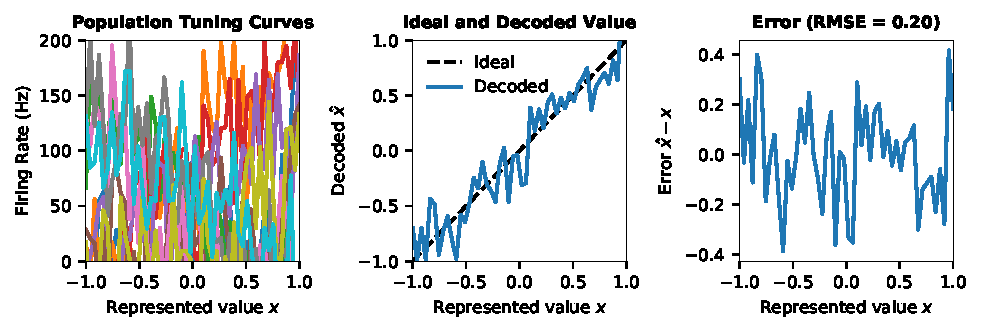
\includegraphics{media/decoding_example_noise_accounted.pdf}
	\caption{Decoding the represented value from a population of neurons with added noise (Gaussian, $\mu = 0$, $\sigma = 0.2 \max(A)$) while accounting for noise. See \cref{fig:decoding_example_no_noise} for the complete description. \CodeLink{lecture_03/media/code/computing_decoders.ipynb}}
	\label{fig:decoding_example_noise_accounted}
\end{figure}

We can now continue to solve for $\vec{d}$ as above. After some linear algebra, we arrive at the following equation (here, directly for arbitrary represented dimensions $d \geq 1$)
\begin{ImportantEqn}{Computing decoders taking noise into account}
	\mat D^\T &\approx  \left(\mat A \mat A^\T + \frac{N \sigma^2}{2} \mat I\right)^{-1} \mat A \mat X^\T \,, \text{ where $\mat I$ is the $n \times n$ identity matrix}
	\label{eqn:decoders_noise}
\end{ImportantEqn}
Adding a scaled version of the identity matrix to $\mat A \mat A^T$ ensures that the resulting matrix is always invertible. If $\sigma^2$ is large enough, this inversion is possible in a numerically stable way. As visible in \cref{fig:decoding_example_noise_accounted}, the decoding error is now in an acceptable range, even if we add noise to the pre-population.

\cprotect\Python{In Python, you can solve the above regularised linear least-squares problem using the following code:
\begin{lstlisting}[language=python]
import numpy as np
A = np.array(...) # n x N array
X = np.array(...) # d x N array
D = np.linalg.lstsq(
        A @ A.T + 0.5 * N * np.square(sigma) * np.eye(n), A @ X.T,
        rcond=None)[0].T
\end{lstlisting}
Using \texttt{lstsq} is numerically more stable than manually inverting the matrix using a function such as \texttt{np.linalg.inv}.}

\Note{Alternative derivation of \cref{eqn:decoders_noise}. The matrix $\mat A \in \mathbb{R}^{n \times N}$ contains samples of neural activities for different represented values. In particular, we have $n$ rows (one for each neuron in the population) for $N$ samples $\vec x_1, \ldots, \vec x_N$ in each row. Furthermore, we assume that there is Gaussian noise superimposed onto our measurements. So we have
\begin{align*}
	\mat A &= \begin{pmatrix}
		a_1({\vec x}_1) + \eta_{1, 1} & \ldots & a_1(\vec x_N) + \eta_{1,N} \\
		\vdots & \ddots & \vdots \\
		a_n({\vec x}_1) + \eta_{n, 1} & \ldots & a_n(\vec x_N) + \eta_{n, N}
	\end{pmatrix} \,, \quad \text{where } \eta_{i, j} \sim \mathcal{N}(0, \sigma^2) \\
	 &= \begin{pmatrix}
	 a_1({\vec x}_1) & \ldots & a_1(\vec x_N) \\
	 \vdots & \ddots & \vdots \\
	 a_n({\vec x}_1) & \ldots & a_n(\vec x_N)
	 \end{pmatrix} + \begin{pmatrix}
	 \eta_{1, 1} & \ldots & \eta_{1,N} \\
	 \vdots & \ddots & \vdots \\
	 \eta_{n, 1} & \ldots & \eta_{n, N}
	 \end{pmatrix} \\
	 &= \mat A_\mathrm{GT} + \mat E \,.
\end{align*}
The matrix $\mat A_\mathrm{GT}$ is a hypothetical matrix of unknown \enquote{ground truth} values and $\mat E$ is the matrix of zero mean Gaussian noise terms. Looking at the term $\mat A \mat A^\T$ from \cref{eqn:decoders} we find
\begin{align*}
	\mat A \mat A^\T
		&= (\mat A_\mathrm{GT} + \mat E) (\mat A_\mathrm{GT} + \mat E)^\T
		 = \mat A_\mathrm{GT}^{} \mat A_\mathrm{GT}^\T + \mat A_\mathrm{GT} \mat E^\T + \mat E \mat A_\mathrm{GT}^\T + \mat E \mat E^\T \,.
\end{align*}
The expectation value of the terms $\mat A_\mathrm{GT} \mat E^\T$ and $\mat E \mat A_\mathrm{GT}^\T$ is zero:
\begin{align*}
	\mathbb{E}\Big[ \big( \mat A_\mathrm{GT}^\T \mat E \big)_{ij} \Big]_{\mat E}
		= \mathbb{E}\Big[ \big( \mat E^\T \mat A_\mathrm{GT} \big)_{ij} \Big]_{\mat E}
		= \mathbb{E}\Big[ \sum_{k = 1}^N a_i(\vec x_k) \eta_{j, k} \Big]_{\mat E}
		= \mathbb{E}\Big[ \sum_{k = 1}^N a_j(\vec x_k) \eta_{i, k} \Big]_{\mat E}
		= 0 \,,
\end{align*}
whereas the term $\mathbb{E}\big[ \mat E^\T \mat E \big]$ evaluates to $N \sigma^2 \mat I$. Hence, for $N \to \infty$ (which, according to the law of large numbers, is bringing us close to the expectation value), we get
\begin{align*}
	(\mat A \mat A^T)^{-1} \mat A \mat X^\T
		&\approx (\mat A^{}_\mathrm{GT} \mat A_\mathrm{GT}^\T + N \sigma^2 \mat I)^{-1} \mat A_\mathrm{GT} \mat X^\T \,.
\end{align*}
Comparing this to \cref{eqn:decoders_noise}, we see that we implicitly assume in \cref{eqn:decoders_noise} that our randomly sampled activities $\mat A$ are equal to the hidden ground truth $\mat A_\mathrm{GT}$, which -- on average -- is correct, since we assume that $\eta_{i,j}$ has a zero mean. We then manually add the term $N \sigma^2 \mat I$, which we would get if we let $N$ go towards infinity -- without actually needing infinitely many samples. Pretty clever, since this saves us a lot of time!

However, the other way round, this derivation shows us that we don't really need to add the term $N \sigma^2 \mat I$ to our sampled activities if only $N$ is large enough (in particular, $N \gg n$).}

\subsection{Analysing Sources of Error}

\begin{figure}
	\centering
	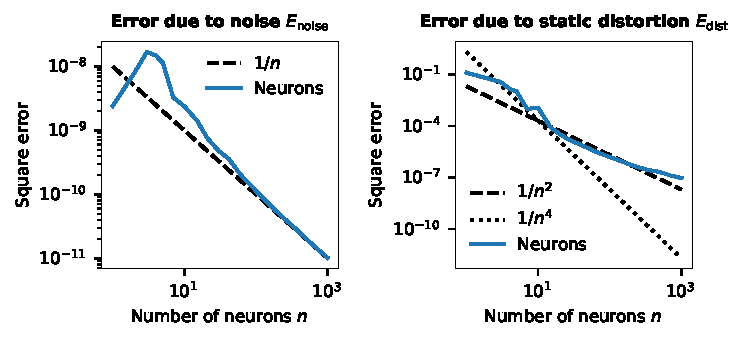
\includegraphics{media/error_experiment.pdf}
	\caption{Error due to noise (\emph{left}) and error due to static distortion (\emph{right}). Experiment for a population of LIF neurons with randomly distributed tuning curves and firing rates between \SIrange{100}{200}{\per\second}, uniform $x$-intercepts over $[-1, 1]$, and $\sigma = 0.01$. \CodeLink{lecture_03/media/code/error_experiment.ipynb}}
	\label{fig:error_experiment}
\end{figure}

We mentioned earlier that neural representations are \emph{lossy}, i.e.,~we cannot perfectly reconstruct the represented value $\vec x$. Looking at our loss function $E$ in \cref{eqn:decoder_loss_regularised}, we see that we modelled the error as caused by two separate effects
\begin{align}
E &= \underbrace{\frac{1}2 \int_{-1}^1 \left(x - \sum_{i = 1}^n d_i a_i(x) \right)^2 \,\mathrm{d}x}_{E_\mathrm{dist}} + \underbrace{\frac{1}2 \sigma^2 \sum_{i = 1}^n d_i^2}_{E_\mathrm{noise}} \,.
\label{eqn:decoder_loss_regularised_sources}
\end{align}
The left term, $E_\mathrm{dist}$, describes errors that are caused by \emph{static distortion}, whereas the right term, $E_\mathrm{noise}$, describes errors due to \emph{noise}.

\paragraph{Errors due to static distortion}
These errors are caused by the shape of the neural tuning curves. Since we assume that the tuning curves are not changing over time, we call this error \enquote{static}. $E_\mathrm{dist}$ is caused by the fact that we are trying to decode the \emph{linear} identity function using a \emph{linear} decoder. Hence, if our tuning curves are, well, \enquote{curved} (such as tuning curves based on LIF neurons), the decoder must somehow eliminate that curvature. The only way to accomplish this for a linear decoder is to find the right weighted average over the tuning curves. However, in general, for randomly distributed tuning curves, there is no way to perfectly decode a linear function from nonlinear tuning curves. Hence, there will always be some degree of error due to static distortion.

\Note{Of course, we can construct edge-case tuning curve distributions in which perfect decoding is possible. For example, consider two ReLU neurons representing a scalar value with encoder $e_1 = 1$ and encoder $e_2 = -1$ (gain and bias are $1$ and $0$ for both neurons, respectively). Then, the decoder $\vec d = (1, -1)$ will perfectly decode the represented value.}

\paragraph{Errors due to noise}
The term $E_\mathrm{noise}$ is giving us an estimate of the amount of error caused by noise, under the assumption that the noise is actually from a Gaussian distribution with variance $\sigma^2$. Intuitively, this error depends on the magnitude of the decoding coefficients -- if all decoding coefficients are zero, noise is effectively eliminated (although, of course $E_\mathrm{distr}$ will be large). The larger the decoding coefficients, the more noise is transported from the neural activities $\vec a$ to the decoded values $\hat{\vec x}$.

\paragraph{Error for varying neuron counts $n$}
Given equation \cref{eqn:decoder_loss_regularised_sources} we can estimate the amount of error caused by static distortion versus the amount of error caused by noise in the neural activities as we change the number of neurons $n$. The (square) error due to noise decreases proportionally to about $1/n$, the error due to distortion decreases proportionally to about $1/n^2$ (cf.~\cref{fig:error_experiment}).

\section{Building a model of a neural population}

With the knowledge we gained above, let's discuss how to practically build a model of a neuron population representing a $d$-dimensional vector $\vec x$. This can be roughly mapped onto the methodology described in \cite{eliasmith2003neural}, Chapter 1.5.

\paragraph{Step 1 and 2: System Description and Design Specification}
First, we have to make a decision regarding the dimensionality $d$ of the quantity $\vec x$ we want to represent, as well as what the range of values $\mathbb{X}$ is. Normally, we define $\mathbb{X}$ as a $d$-dimensional hyper-ball with radius $r$, that is $\mathbb{X} = \big\{ \vec x \mid \| \vec x \| \leq r, \vec x \in \mathbb{R}^d \big\}$ (typically $r = 1$).

Furthermore, we have to specify how many neurons $n$ are in the population, and what their tuning curves are. This will have an impact on the precision with which the values are represented. The tuning curves will determine the parameters we choose for $\alpha_i$, $J^\mathrm{bias}_i$, $\vec e_i$.

In case we have no specific information about the tuning curves, we select these parameters for each neuron in the population such that
\begin{itemize}
	\item The encoders $\vec e_i$ should be uniformly sampled from the unit-sphere. This can be achieved by sampling each encoder component from a normal distribution (i.e.,~a Gaussian distribution with mean zero and variance one) and normalising the resulting vectors to length one.
	\item The maximum neural firing rate is limited to the maximum rate we observe in biology. The maximum firing rate is the rate we get when the represented value $\vec x$ is aligned with the encoding vector $\vec e_i$, i.e.~$\langle \vec x, \vec e_i \rangle = r$. Typically, the maximum firing rates of a population should be uniformly distributed between \SIrange{100}{200}{\per\second}. Per default, Nengo uses a maximum firing rate range between \SIrange{200}{400}{\per\second}, which is typically to large for most brain regions.
	\item The $x$-intercepts, i.e.~the value of $\langle \vec x, \vec e_i \rangle$ at which the neuron just starts to have a nonzero activity should be uniformly sampled from $[-r, r]$.
\end{itemize}

\paragraph{Step 3: Implementation}
After we have chosen the parameters above, we can encode values $\vec x$ in the population. In other words, we can take an $\vec x$ and compute the neural population response $\vec a(\vec x)$ according to the encoding equation. We can then uniformly sample $N$ samples $\vec x_1, \ldots, \vec x_N$ from $\mathbb{X}$ and compute neural activation matrix $\mat A$.

Finally, this allows us to compute the decoders $\mat D$ according to \cref{eqn:decoders_noise}, where $\sigma$ depends on the amount of noise we expect in the neural activities. As a rule of thumb, a value of $\sigma = 0.2 \max\{\mat A\}$ is a good starting point.

\Note{This might all still seem a little abstract -- for this reason, you will implement all these steps in Assignment 1.}

\subsection{Example: Horizontal Eye Position (1D)}

\begin{figure}
	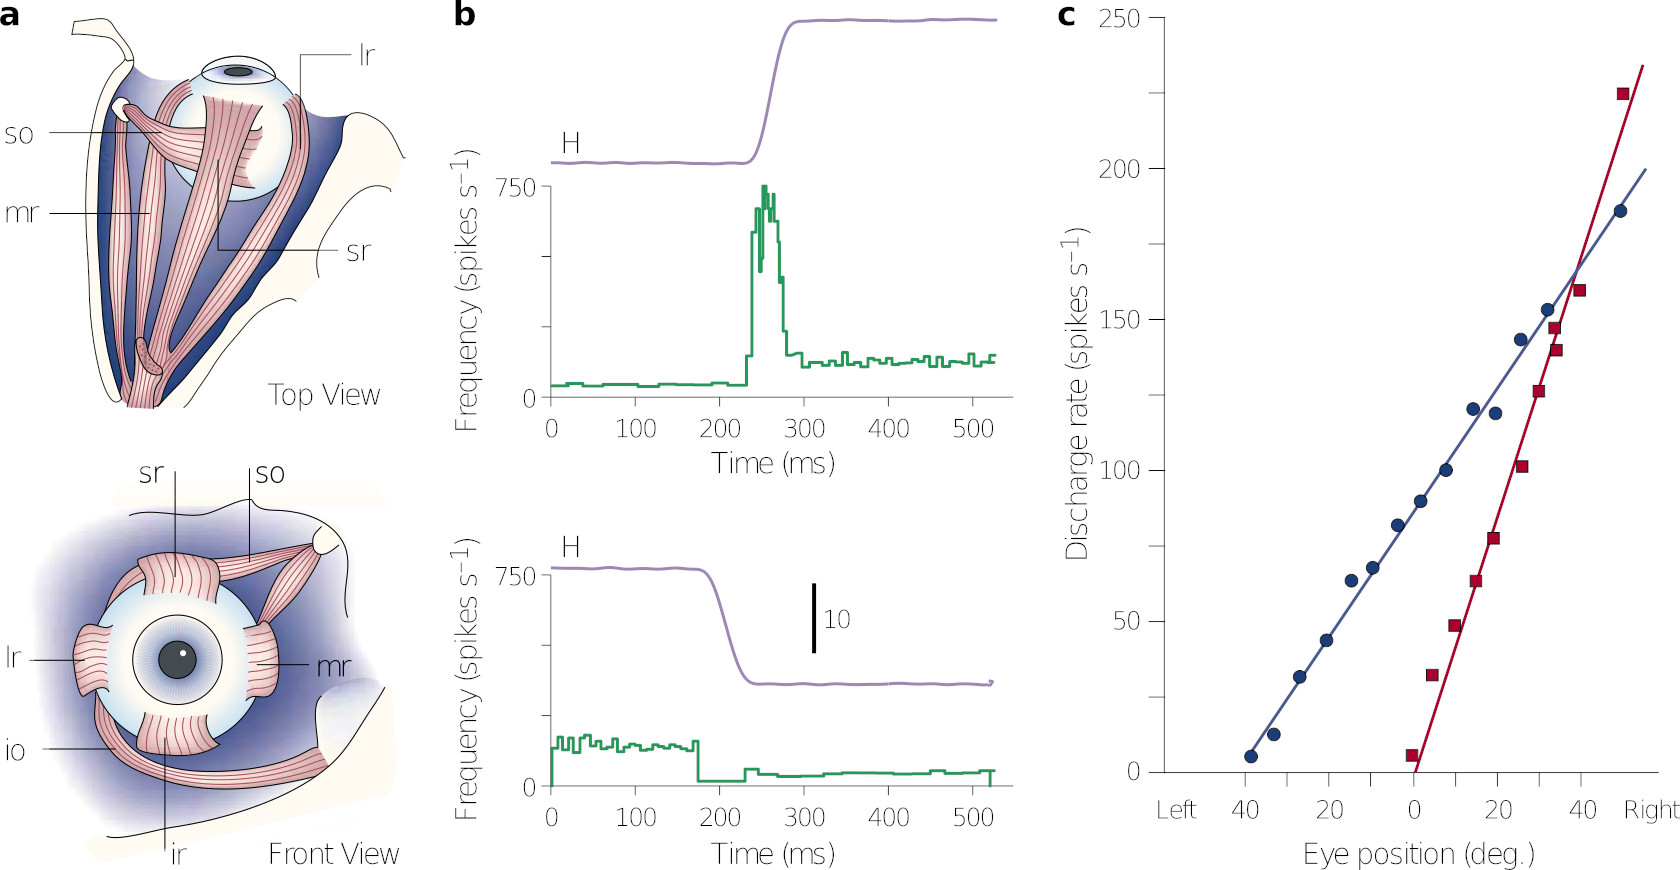
\includegraphics{media/sparks_et_al_2002_brainstem_eye.jpg}
	\caption{Extraocular muscles and typical activity of motor neurons. \textbf{(a)} Anatomical drawing of the muscles controlling eye position. \textbf{(b)} Neural activity and eye position over time. \textbf{(c)} Neural activity over eye position for two abducens motor neurons. There is a linear relationship between eye position and firing rate. Caption and figure copied from \cite{sparks2002brainstem}.}
	\label{fig:sparks_et_al_2002_brainstem_eye}
\end{figure}

\Cref{fig:sparks_et_al_2002_brainstem_eye} is taken from a review paper on the neural circuits involved in eye position control \cite{sparks2002brainstem}. The depicted neural activities show the firing rates of neurons forming the abducens nerve, which is directly connected to the muscles controlling eye location. As visible in the figure, there is an almost linear relationship between the eye position (in degrees) and the neural activity. In addition to neurons exhibiting a positive relationship between eye position and firing rate (\enquote{on} neurons), there are also neurons with the opposite relationship (\enquote{off} neurons).

\begin{figure}
	\centering
	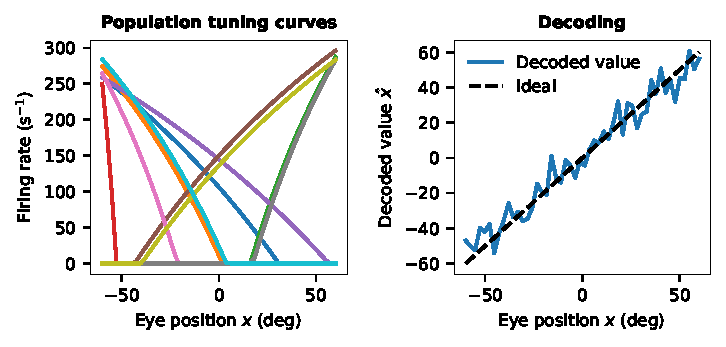
\includegraphics{media/1d_eye_position.pdf}
	\caption{Model of eye position representation. \emph{Left:} Population tuning curves. \emph{Right:} Ideal versus actual decoding under noise. \CodeLink{lecture_03/media/code/1d_eye_position.ipynb}}
	\label{fig:1d_eye_position}
\end{figure}

We can now go through the three steps described above and try to build a neural ensemble that represents eye location. See \cref{fig:1d_eye_position} for an example.
\begin{multicols}{2}
\begin{itemize}
	\item \textbf{Step 1: System Description}
	\begin{itemize}
		\item What is being represented?
		\begin{itemize}
			\item Represented quantity $x$ is the horizontal eye position
		\end{itemize}
		\item What do the tuning curves look like?
		\begin{itemize}
			\item Extremely linear, low $\tau_\mathrm{ref}$, high $\tau_\mathrm{RC}$
			\item Some neurons have $e = 1$, others have $e = -1$
			\item Firing rates up to \SI{300}{\per\second}
		\end{itemize}
	\end{itemize}
	\columnbreak
	\item \textbf{Step 2: Design Specification}
	\begin{itemize}
		\item Range of values
		\begin{itemize}
			\item $\mathbb{X} = [-60, 60]$
		\end{itemize}
		\item Amount of noise
		\begin{itemize}
			\item About $20\%$ of the maximum firing rate, hence $\sigma^2 = 0.04$
		\end{itemize}
	\end{itemize}
	\item \textbf{Step 3: Implementation}
	\begin{itemize}
		\item Choose parameters that determine the tuning curves
		\item Compute decoders
	\end{itemize}
\end{itemize}
\end{multicols}

\subsection{Example: Arm Movements (2D)}

\begin{figure}
	\begin{subfigure}{0.5\textwidth}
		\centering
		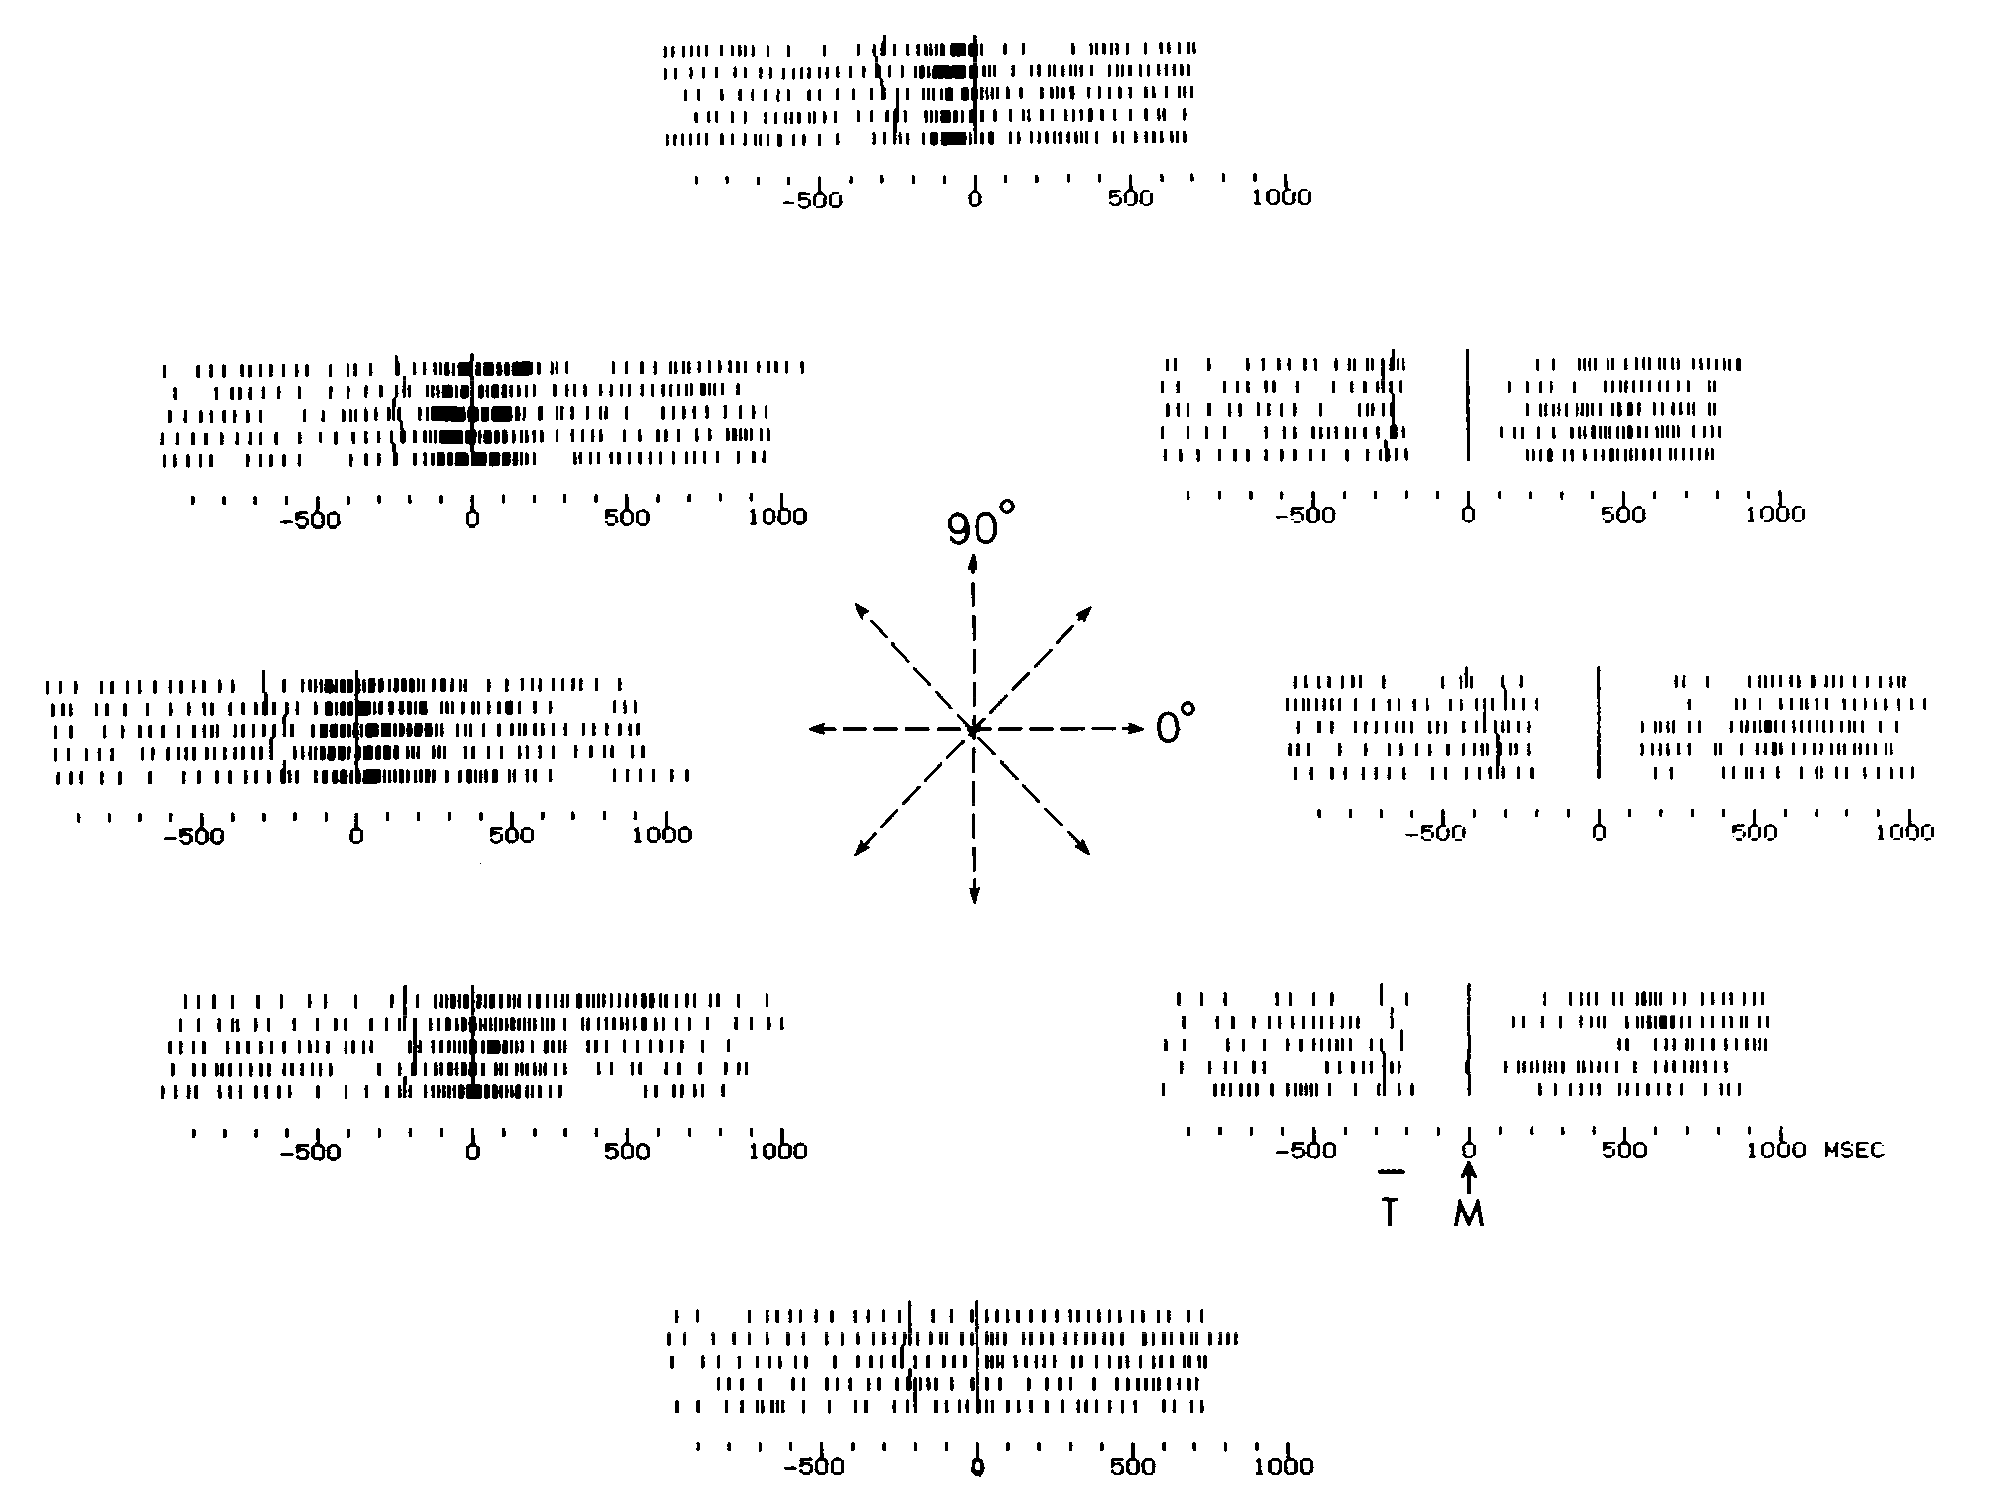
\includegraphics[width=\textwidth]{media/georgopoulos_spike_raster.png}
		\caption{Spike rasters for different movement directions}
		\label{fig:georgopoulos_a}
	\end{subfigure}
	\begin{subfigure}{0.5\textwidth}
		\centering
		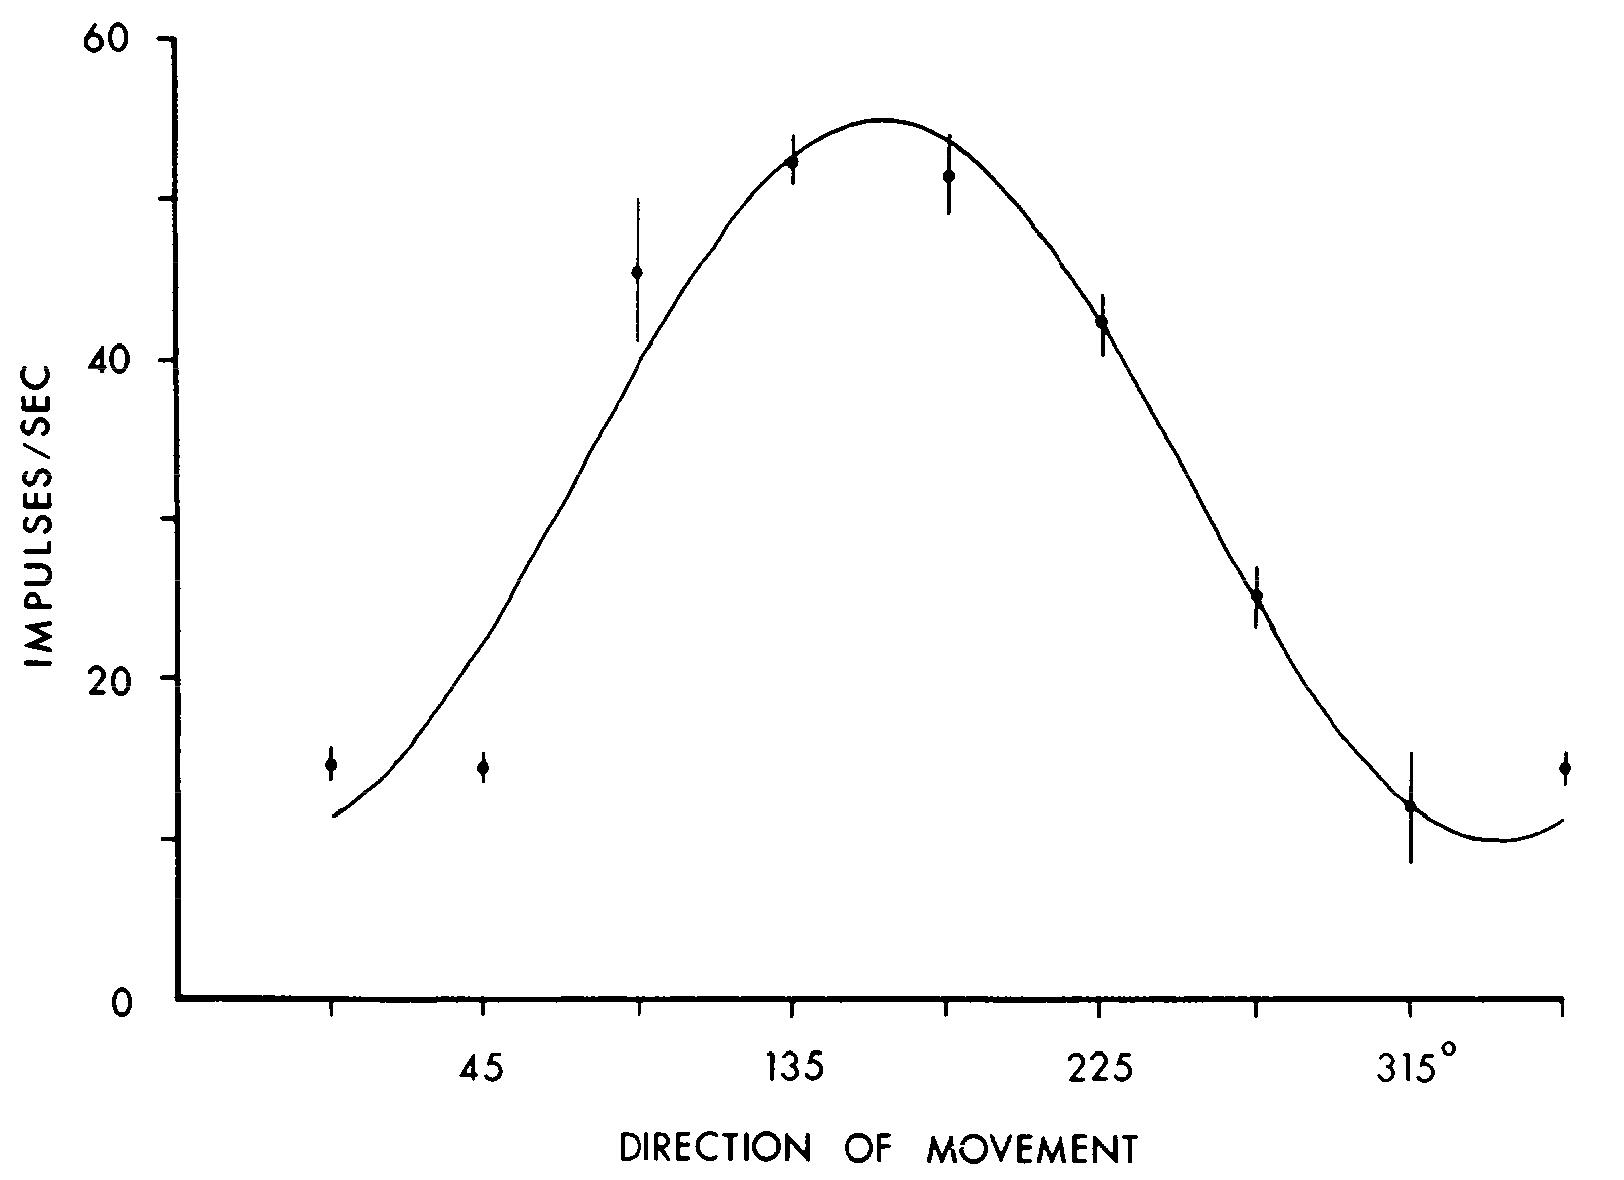
\includegraphics[width=\textwidth]{media/georgopoulos_tuning.png}
		\caption{Single neuron tuning curve}
		\label{fig:georgopoulos_b}
	\end{subfigure}
	\caption{Experiment by Georgopoulos et~al, 1982. Diagram shows recordings from a single cell in motor cortex representing direction of hand movement and/or hand position. \textbf{(a)} Recordings from the same cell in motor cortex over different trials. The individual sections correspond to a monkey moving their hand from a centre location into one of eight directions. \textbf{(b)} Averaged tuning curve over different directions with a sine fit. Figures copied from \cite{georgopoulos1982relations}.}
	\label{fig:georgopoulos}
\end{figure}

\begin{figure}
	\begin{subfigure}[b]{0.5\textwidth}
		\centering
		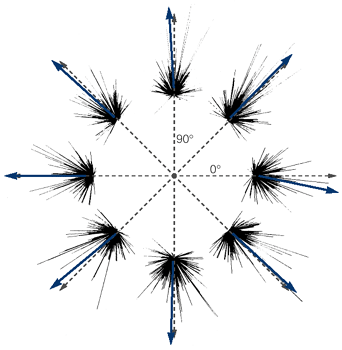
\includegraphics[width=0.7\textwidth]{media/georgopoulos_directions.png}
		\caption{Population vectors}
		\label{fig:population_vector}
	\end{subfigure}
	\begin{subfigure}[b]{0.5\textwidth}
		\centering
		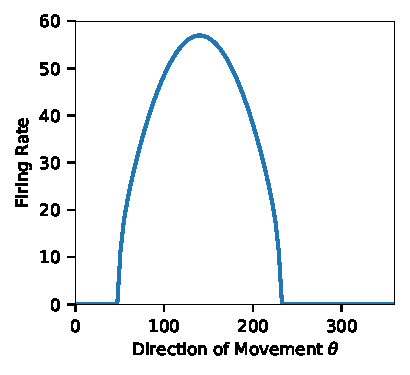
\includegraphics{media/2d_tuning.pdf}
		\caption{Tuning curve model}
		\label{fig:georgopoulos_model}
	\end{subfigure}
	\caption{\textbf{(a)} Visualisation of the concept of a population vector. Each neuron (black lines) has a preferred direction. The magnitude of the neural activity while the animal is moving their arm into a certain direction corresponds to the length of the black line. Georgopoulos decodes the motion direction from the population by computing the average of the preferred direction vectors, weighted by the neural activity of the corresponding neurons. In NEF terminology, this corresponds to using the matrix of encoders $\mat E$ as decoders $\mat D$. \textbf{(b)} Model of the movement direction tuning curve modelled in the NEF. \CodeLink{lecture_03/media/code/2d_arm_movement.ipynb}}
\end{figure}

\Cref{fig:georgopoulos_a} shows data from a experiment by Georgopoulos et~al., in which neural activity in motor cortex is recorded while a monkey is moving their hand into one of eight directions. The neural activity is found to be highly correlated with the direction of movement, with individual neurons having a clear \enquote{preferred direction} (\cref{fig:georgopoulos_b}). This gave rise to the idea of a \enquote{population vector}, i.e.,~that the represented vector of the population is the average of the preferred directions, weighted by the neural activities (\cref{fig:population_vector}).

\Note{While conceptually similar (i.e.,~there is a linear decoding scheme), the NEF does \emph{not} use \enquote{population vectors} in order to represent vectorial quantities¸ -- in particular, the decoding process is different. Georgopulos essentially uses the encoders (i.e.,~the preferred directions) as decoders (cf.~\cref{fig:population_vector}):
\begin{align*}
	\hat{\vec x} \approx \sum_{i = 1}^n a_i(\vec x) \vec e_i = \mat E \mat A 
\end{align*}	
This gives a reasonable estimate of the direction, but a terrible estimate of the magnitude of the represented vector. In the NEF, we essentially assume that there is some correlation between the represented value and the activity, and the decoders is used to decipher that encoded value from the population activities.}

Again, we can model this system using the NEF Principle 1. A single tuning curve that has been modelled in this way is depicted in \cref{fig:georgopoulos_model}.
\begin{multicols}{2}
	\begin{itemize}
		\item \textbf{Step 1: System Description}
		\begin{itemize}
			\item What is being represented?
			\begin{itemize}
				\item $\vec x$ the movement direction (or hand position)
			\end{itemize}
			\item What do the tuning curves look like?
			\begin{itemize}
				\item Bell-shaped
				\item Encoders are randomly distributed along the unit circle
				\item Firing rates up to \SI{60}{\per\second}
			\end{itemize}
		\end{itemize}
		\columnbreak
		\item \textbf{Step 2: Design Specification}
		\begin{itemize}
			\item Range of values
			\begin{itemize}
				\item $\mathbb{X} = \{\vec x \mid \|\vec x\| \leq r, \vec x \in \mathbb{R}^2 \}$
			\end{itemize}
			\item Amount of noise
			\begin{itemize}
				\item About $20\%$ of the maximum firing rate
			\end{itemize}
		\end{itemize}
		\item \textbf{Step 3: Implementation}
		\begin{itemize}
			\item Choose parameters that determine the tuning curves
			\item Compute decoders
		\end{itemize}
	\end{itemize}
\end{multicols}

\subsection{Example: Higher-dimensional Tuning}

\begin{figure}
	\begin{subfigure}[b]{0.5\textwidth}
		\centering
		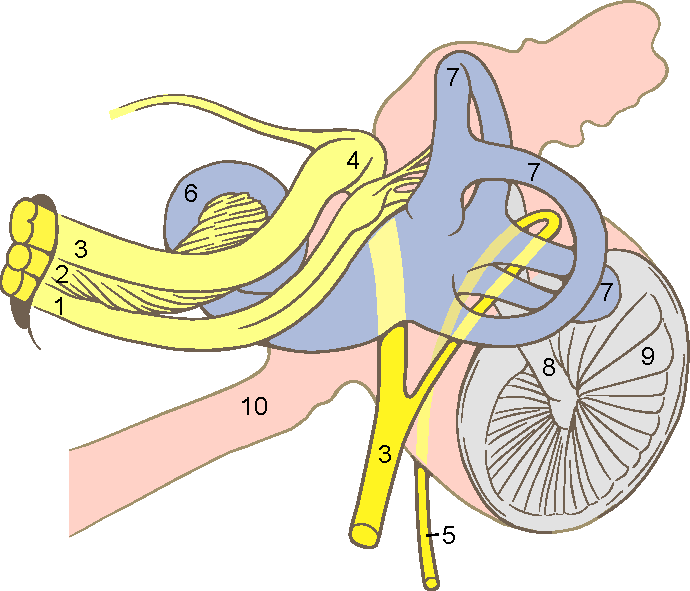
\includegraphics[width=0.85\textwidth]{media/ear_internal_anatomy_numbered.pdf}
		\caption{Inner ear anatomy}
		\label{fig:ear_internal_anatomy_numbered}
	\end{subfigure}
	\begin{subfigure}[b]{0.5\textwidth}
		\centering
		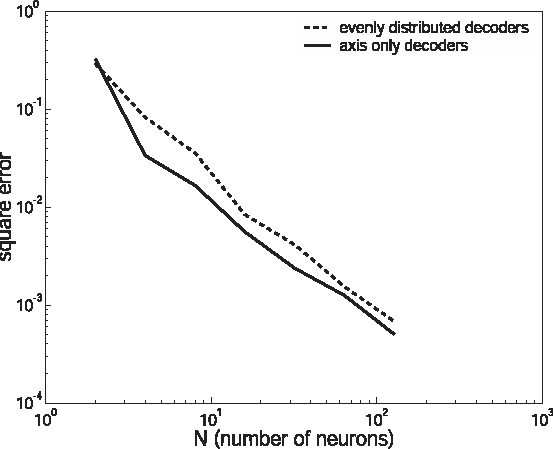
\includegraphics[width=\textwidth]{media/eliasmith_et_al_2003_axis_aligned.pdf}
		\caption{Axis-aligned versus uniform encoders}
		\label{fig:eliasmith_et_al_2003_axis_aligned}
	\end{subfigure}
	\caption{\textbf{(a)} Anatomy of the inner ear. (1) Nervus vestibularis, (2) Nervus cochlearis, (3) Nervus intermediofacialis, (4) Ganglion geniculi, (5) Chorda tympani, (6) Cochlea, (7) Ductus semicirculares, (8) Malleus, (9) Membrana tympani, (10) Tuba auditiva. Figure from \href{https://commons.wikimedia.org/wiki/File:Ear_internal_anatomy_numbered.svg}{Wikimedia}, by Patrick J. Lynch. \textbf{(b)} Difference between modelling multi-dimensional ensembles with axis aligned vectors or uniformly distributed encoders.}
\end{figure}

While we assumed in the previous example that encoders are randomly distributed, this is not necessarily the case. For example, take the vestibular system, i.e.,~the part of the inner ear responsible for sensing head acceleration \cref{fig:ear_internal_anatomy_numbered}. This system consists of three orthogonal canals (the \enquote{semicircular canals}), each detecting movement along one spatial dimension.  We could correspondingly model the sensory system as a population of neurons representing a three-dimensional quantity, namely the direction into which the head is accelerating. However, it would be biologically implausible to choose random preferred directions, i.e.~encoders. Due to the physical properties of the organ, the preferred directions of the individual neurons are axis aligned, we have encoders of the form
\begin{align*}
	\vec e_i \in \big\{ [1, 0, 0], [-1, 0, 0], [0, 1, 0], [0, -1, 0], [0, 0, 1], [0, 0, -1] \big\} \,.
\end{align*}
This is equivalent to just using three independent one-dimensional neuron populations. In general, the choice of the encoders affects the representation accuracy: axis-aligned encoders result in a lower accuracy compared to encoders uniformly sampled from the unit sphere. (\cref{fig:eliasmith_et_al_2003_axis_aligned}).


\printbibliography

\end{document}
